

\chapter{Molecular Vibrations}

\textit{Berechnen sie den Huang Rhys Faktor 
}
\textit{Evtl. Testen sie das Spiegel-Gesetz.
}


% \section{Experiment}

section{4.2. Stokes-Verschiebung und Spiegel-Regel\protect\footnote{Parson, Kap. 5.2 und 5.3, Simon Biberger}\hfill ***} 

\textit{Wie kommt es zu den Unterschieden und Gemeinsamkeiten
zwischen Absorption und Emission?}\\
Unter Stokes-Shift versteht man die Unterschiede in der Energie bei Absorption und Emission. Dabei tritt die Emission immer bei längeren Wellenlängen bzw. kleineren Energien als die Absorption auf. Da die vibronische Relaxation immer eine kleinere Lebenszeit als die elektronischen Übergänge besitzt, finden sowohl Absorption als auch Emission von niedrigsten Schwingungszustand des elektronischen Niveaus statt. (Kasha's Rule)

\begin{figure}[htb]
    \centering
    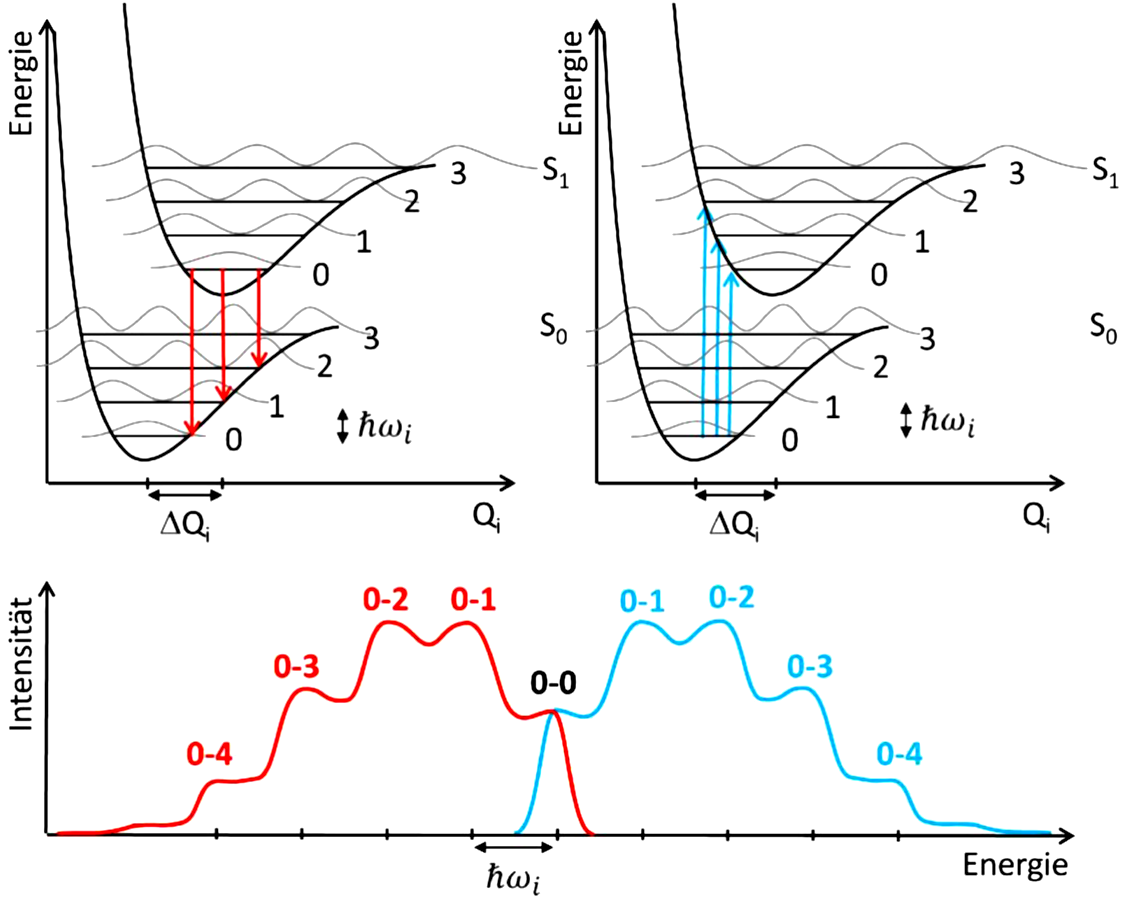
\includegraphics[width = 0.9 \textwidth]{\currfiledir/Stokes.png}
    \caption{Absorption (blau) und Emission (rot). Die Potentialkurven zeigen die elektronischen Niveaus. Zusätzlich sind die Schwingungszustände $\nu$ mit den jeweiligen Quantenzahlen eingezeichnet. Mit den Pfeilen sind mögliche Absorptions- und Emissionsvorgänge markiert}
    \label{Stokes}
\end{figure}

Neben dem Einfluss der vibronischen Relaxation gibt es in Lösung zusätzlich den Solvent Stokes-Shift. Hierbei gibt das Molekül Energie an die Umgebung ab, bevor es zum Übergang kommt. Im Idealfall haben das Absorptions- und Emissionsspektrum dieselbe Struktur, wie es in Abbildung \ref{Stokes} gezeigt ist. Für diesen Fall müssen einige Voraussetzungen erfüllt sein:\protect\footnote{Warum werden, wie im Parson auf Seite 231 gezeigt, Absorption mit $\nu^{-1}$ und die Emission mit $\nu^{-3}$ gewichtet}

\begin{itemize}
    \item korrespondierende Übergänge haben gleiche Frank-Condon-Faoren
    \item Born-Oppenheimer-Näherung ist gültig
    \item Schwingungsmoden sind harmonisch und besitzen feste Frequenzen
    \item Schwingungswellenfunktionsüberlapp für Absorption und Emission ist gleich groß
    \item Die Schwingungsniveaus von Grundzustand und angeregtem Zustand sollten auch gleich stark bevölkert sein
\end{itemize}

Bei Abweichung von diesen Bedingungen ist die Spiegel-Symmetrie gebrochen und Emission findet bei leicht höheren Energien, wie sie die Spiegel-Symmetrie vorhersagt, statt.



\section{5.4. Normalmoden\protect\footnote{Parson, Kap. 6.1, Daniel Kroh}\hfill *} 
Wie läßt sich die Bewegung der Atome in Molekülen
beschreiben?  Wieder ignorieren wir hier die volle
Gruppentheorie. \newline
Die Anregung von Molekülen in höhere vibronische Zustände erfolgt im mittleren Infrarotbereich ($\lambda = 2,5-50 \mu m$). Ein Molekül mit N Atomen hat hierbei 3N Bewegungsfreiheitsgrade. Wobei 3 zu der Translation aus dem Masseschwerpunkt gehören, 3 zu der Rotation des ganzen Moleküls und (3N-6) zu internen Vibrationen, die den Massenschwerpunkt stationär halten. Allgemein gilt, dass jede Vibrationsmode eines komplexen Moleküls die kollektive Bewegung vieler Kerne beeinhaltet und nicht so einfach beschrieben werden kann, wie das Stauchen und Strecken einer einzelnen Bindung. Zur Vereinfachung nehmen wir an, dass das Vibrationspotential eine harmonische Funktion der Atomkoordinaten ist, d.h. das Potential hängt von quadratischen Termen wie $x_i^2$, $x_ix_j$ (mit $x_i$,$x_j$ als Auslenkung in jede der 3N kartesischen Koordinaten aus der Ruhelage), aber nicht von Termen höherer Ordnung ab! Mit dieser Annahme ist es möglich orthogonale Normalkoordinaten aus Linearkomtinationen der einzelnen Atomkoordinaten zu definiere, so dass jede vibronische Mode (Normalmode) nur Bewegung entlang einer Normalkoordinate beinhaltet.\\

Das Vibrationspotential eines Moleküls lässt sich somit schreiben als
\begin{equation}
    V = \frac{1}{2} \sum_i k_i \zeta_i^2
\end{equation}
wobei $\zeta_i$ die Normalkoordinate für die Mode i und $k_i$ eine Kraftkonstante für diese Bewegung ist. \\
Die Lösungen der Schrödingergleichung für ein quadratisches Potential als Funktion der Koordinate x sind die Wellenfunktionen eines harmonischen Oszillators:
\begin{equation}
    \chi_n = N_n H_n(u) exp(-u^2/2)
\end{equation}
mit der dimensionslosen Koordinate $u = x/(\hbar/2\pi m_r\nu)^{1/2}$, der reduzierten Masse des Systems $m_r$, der klassischen Schwinungsfrequenz $\nu$, dem Hermite-Polymnom $H_n(u_i)$ und dem Normalisierunsfaktor $N_n$. \\
Die Frequenz eines harmonischen Oszillators mit Kraftkonstante $k_i$ ist gegeben durch:
\begin{equation}
    \nu = (k/m_r)^{1/2}/2\pi
\end{equation}
Innerhalb der Grenzen der harmonischen Näherung ist eine vibronische Wellenfunktion eines nicht-linearen Moleküls einfach das Produkt der Wellenfunktionen der (3N-6) unabhängigen harmonischen Oszillatoren:
\begin{equation}
    X(x_1, x_2, ...) = \prod_{i=1}^{3N-6} \chi_{i(n)}(x_i)
\end{equation}
Und mit der gleichen Näherung ist die Schwinungsenergie eines Moleküls die Summe der Energien einer einzelnen Normalmode:
\begin{equation}
    E_{vib} = \sum_{i=1}^{3N-6}(n_i + \frac{1}{2})h\nu_i,
\end{equation}
wobei $n_i$ das Anregungslevel der Mode $i$ ist. \\
Abbildung \ref{fig_Normalmoden} zeigt die Normalmoden eines linearen und nicht-linearen dreiatomigen Moleküls. Auch wenn die Normalmoden von größeren Molekülen deutlich komplizierter sein können und meist Bewegungen vieler Atome beinhalte, können manche Moden dennoch als gemeinsame Bewegung kleinerer Gruppen von Atomen beschrieben werden.
\begin{figure}[htb]
    \centering
    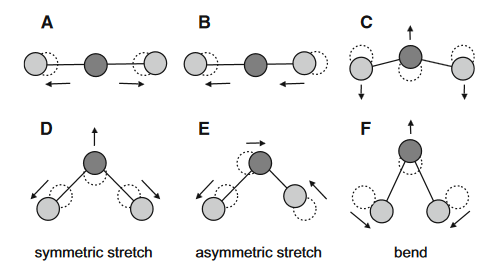
\includegraphics[width = 1 \textwidth]{\currfiledir/Normalmoden.png}
    \caption{Normalmoden eines linearen (A-C) und nicht-linearen (D-F) dreiatomigen Moleküls. Die gestrichelten und gefüllten Kreise stellen Positionen der Atome bei zwei Extrema der Bewegung dar; Pfeile zeigen die Bewegungen in eine Richtung zwischen diesen Extrema. Biegen und sysmmetrisches Dehnen erhalten die Spiegelsymmetrie, wobei das asymmetrische Dehnen die Symmetire zerstört. Ein lineares dreiatomiges Molekül hat zudem eine Zusätzliche Dehungsmode senkrecht zur Zeichenebene, aber besitzt nur zwei Rotationsmoden, wobei ein nicht-lineares Molekül drei besitzt. Beide haben zudem eine einzige Translationsmode}
    \label{fig_Normalmoden}
\end{figure}
\section{5.5. Anregung von Schwingungsmoden\protect\footnote{Parson, Kap. 6.2}\hfill **} 

Welche Schwingungsmoden wechselwirken mit  Licht? Das
Ergebnis kennen sie aus dem 5. Semester. Die Herleitung ist
hier schöner.

Analog zu den Übergängen zwischen elektronischen Energieniveaus kann auch für Übergänge zwischen den Schwingungsniveaus mit den Wellenfunktionen $\chi_{m}$ und $\chi_{n}$ ein Übergangsdipol
\begin{equation}
    \vec{\mu}_{mn} = \Braket{\chi_{m} | \vec{\mu} | \chi_{n}}
\end{equation}
definiert werden. Zur Vereinfachung wird zunächst von einem zweiatomigen Molekül ausgegangen, welches nur eine Schwingungs-Normalkoordinate $x$ besitzt. Das Dipolmoment $\vec{\mu}$ kann dann um die Ruhelage $x = 0$ entwickelt werden:
\begin{equation}
    \vec{\mu}(x) = \vec{\mu}(0) + \frac{\partial \vec{\mu}}{\partial x}\Bigr|_{x=0} x + \dots
\end{equation}
Für den Übergangsdipol gilt dann
\begin{equation}
    \vec{\mu}_{mn} = \vec{\mu}(0) \Braket{\chi_{m} | \chi_{n}} + \frac{\partial \vec{\mu}}{\partial x}\Bigr|_{x=0} \Braket{\chi_{m} | x | \chi_{n}} + \dots .
\end{equation}
Der erste Summand ist Null, da die Wellenfunktionen der Schwingungsniveaus orthogonal sind. Damit der Übergangsdipol nicht verschwindet, muss somit gelten:
\begin{enumerate}
    \item $\frac{\partial \vec{\mu}}{\partial x}\Bigr|_{x=0} \neq 0$. Ein Übergang zwischen den Schwingungsniveaus in \ch{O2} ist also beispielsweise verboten, weil das Dipolmoment symmetriebedingt verschwindet.
    \item $\Braket{\chi_{m} | x | \chi_{n}} \neq 0$. Dies ist beim harmonischen Oszillator der Fall, wenn $m - n = \pm 1$. Es sind somit nur Übergänge zwischen benachbarten Schwingungsniveaus erlaubt.
\end{enumerate}
Aufgrund der Nichtlinearität des Potentials besitzen im Allgemeinen auch Übergänge $m - n = \pm 2, \pm 3, \dots$ einen nicht verschwindenden Übergangsdipol, dessen Betrag aber mit steigender Ordnung immer kleiner wird. Für Moleküle mit mehr als zwei Atomen muss die oben durchgeführte Taylor-Entwicklung auf mehrere Dimensionen, entsprechend den Normalkoordinaten, erweitert werden.




\printbibliography[segment=\therefsegment,heading=subbibliography]
